%Anwendungsfalldiagramme
\section{Anwendungsfall-Diagramme}
Anwendungsfälle und Aktivitätsdiagramme bezüglich der Funktionen der Schnittstelle. Hierbei wird sich an den Testfällen orientiert und einige Testszenarien zusammengefasst.

Anwendungsfall für den Besuch der Schnittstelle
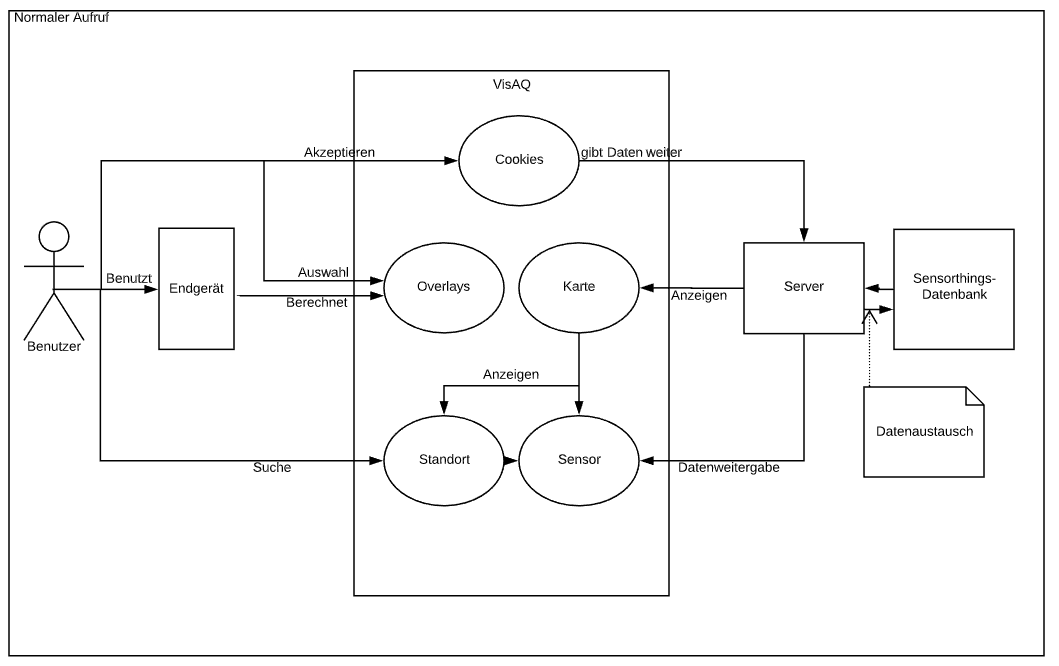
\includegraphics[width=0.9\textwidth]{media/Anwendungsfall1}\captionof{figure}{Anwendungsfall normaler Nutzer} 

Aktivitätsdiagramm für die Auswahl der Modi: Farbblindheit, Dark Mode und Expertenmodus
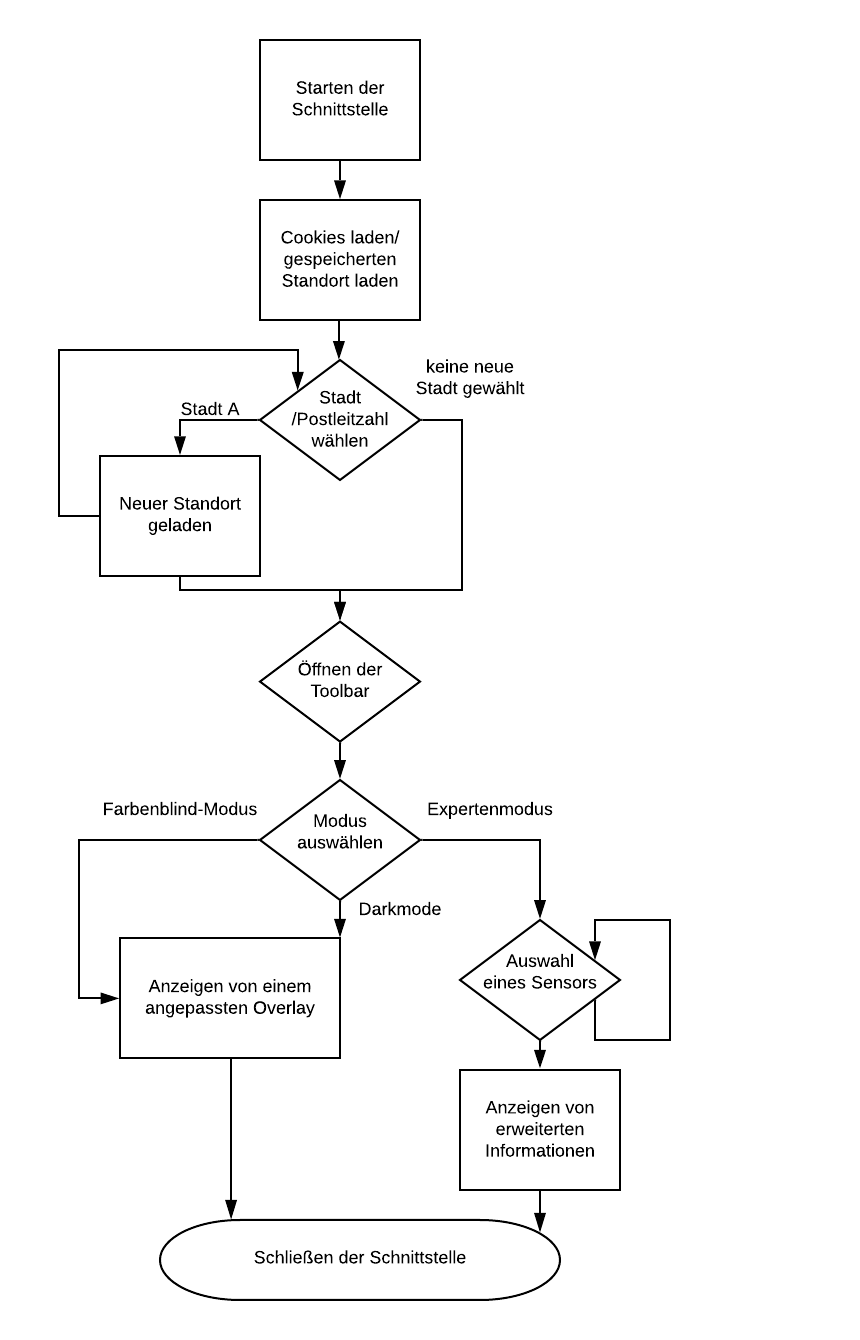
\includegraphics[width=0.9\textwidth]{media/AuswahlModi}\captionof{figure}{Auswahl der unterschiedlichen Modi} 

Aktivitätsdiagramm für die Auswahl der Sensoren und/oder Auswahl eines interpolierten Standpunktes auf der Karte
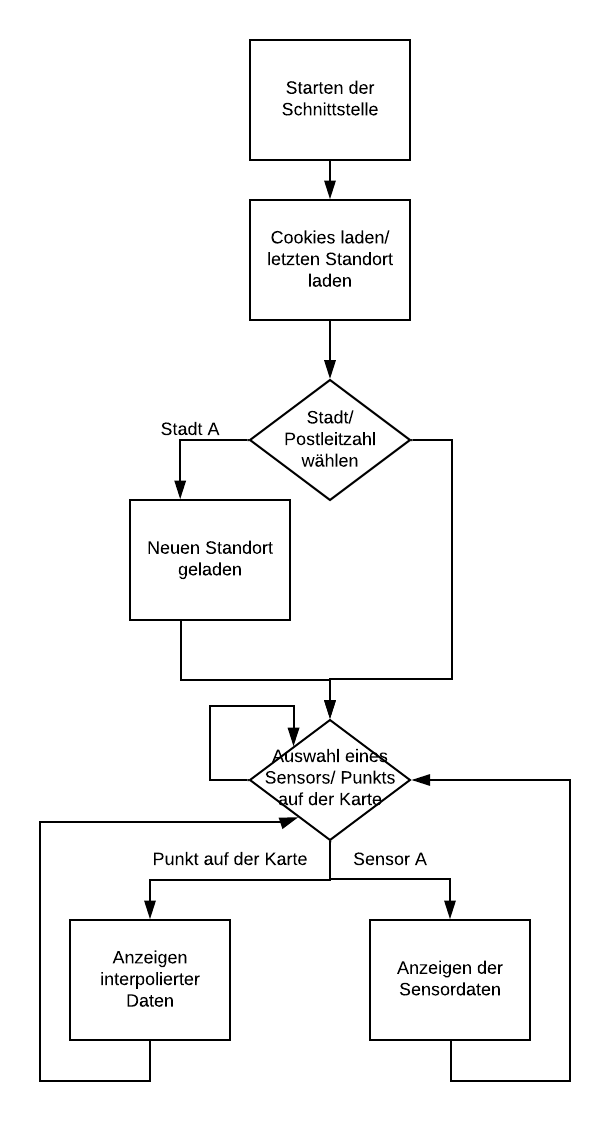
\includegraphics[width=0.9\textwidth]{media/AuswahlSensoren}\captionof{figure}{Auswahl unterschiedlicher \glspl{Sensor} und interpolierter Standpunkte} 

Aktivitätsdiagramm zu der Auswahl der unterschiedlichen Kartenoverlays
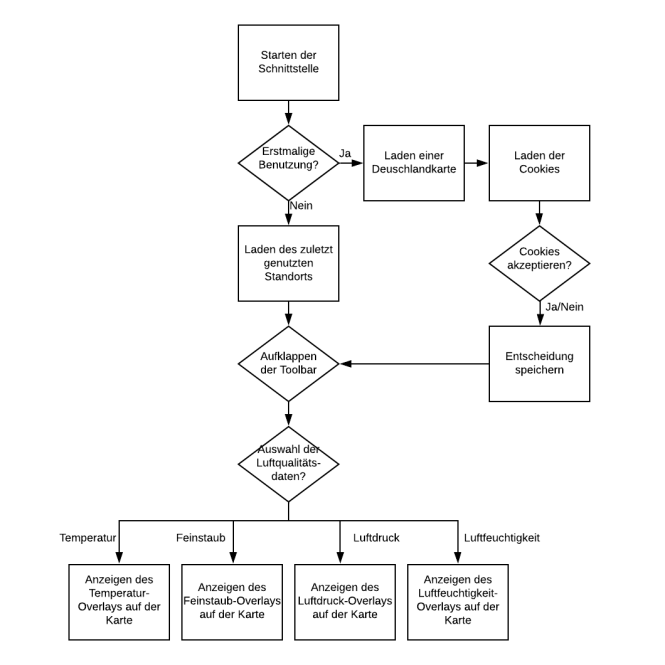
\includegraphics[width=0.9\textwidth]{media/Overlays}\captionof{figure}{Auswahl der unterschiedlichen Overlays} 

Aktivitätsdiagramm zu einer fehlerhaften Eingabe der Stadt beziehungsweise Postleitzahl in der Suchleiste
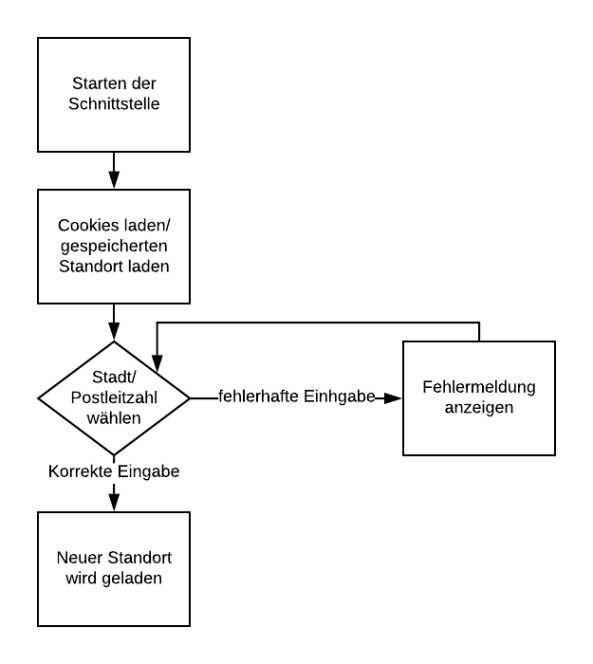
\includegraphics[width=0.9\textwidth]{media/Fehlerhafte-Eingabe}\captionof{figure}{Fehlerhafte Eingabe} 

Öffnen der zeitlichen Entwicklung über die Toolbar und bedienen dieser mittels eines Schiebebalken
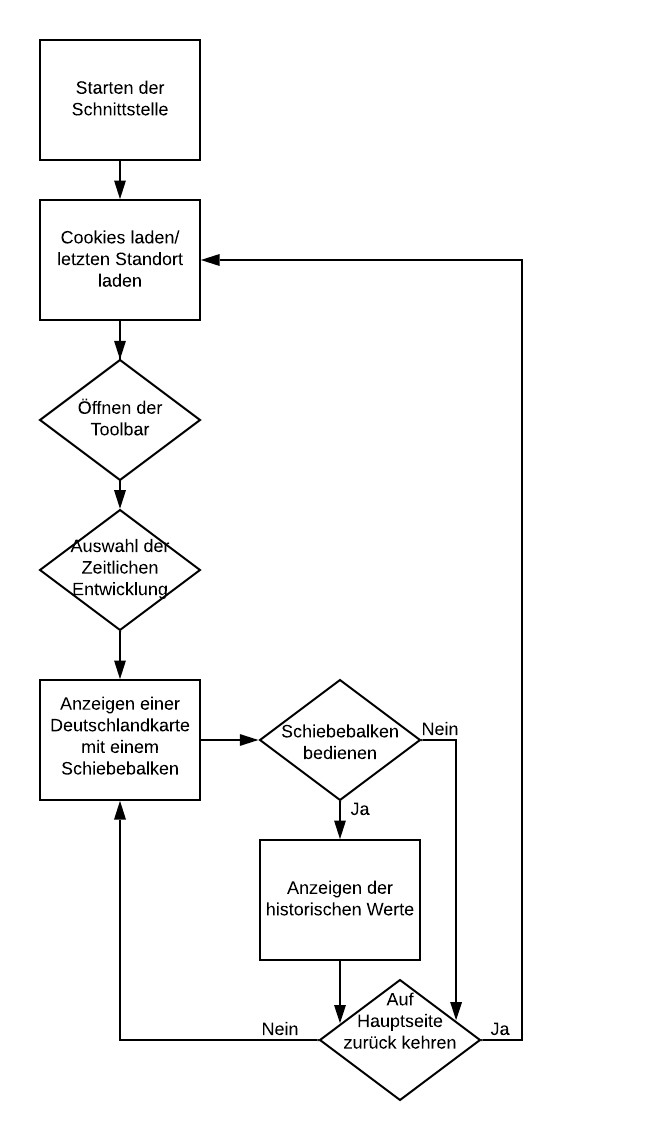
\includegraphics[width=0.9\textwidth]{media/Zeitliche-Entwicklung-Diagramm}\captionof{figure}{Zeitliche Entwicklung} 